

\chapter{Fundamentação Teórica}
\label{cap:fundamentacao-teorica}

Esta seção explora as principais teorias, conceitos e tecnologias relevantes para o desenvolvimento e a aplicação de técnicas de Inteligência Artificial (IA) e engenharia de prompt (prompting) no contexto da automação de documentos jurídicos.

Para compreender de forma mais aprofundada os modelos utilizados, os comportamentos observados e as estratégias de interação adotadas, torna-se essencial retomar os fundamentos teóricos e conceituais que sustentam os modelos de IA generativa. Inicialmente, serão apresentados os conceitos basilares de Inteligência Artificial (IA), Aprendizagem de Máquina (AM), Processamento de Linguagem Natural (PLN) e Engenharia de Prompt. Em seguida, direciona-se o foco para as técnicas e estruturas subjacentes aos modelos explorados neste trabalho.

Conceitos como Redes Neurais Artificiais (RNA), Aprendizagem Profunda (AP), mecanismos de atenção, especialmente a arquitetura Transformer, são fundamentais para a compreensão do funcionamento dos Modelos de Linguagem de Larga Escala (LLM) empregados no processo de automação aqui proposto. Esses modelos, amplamente utilizados em tarefas de geração textual, tradução automática e resumo de documentos, são capazes de captar relações contextuais complexas, mesmo em textos longos e com múltiplos interlocutores, como é o caso das transcrições de reuniões.

\section{Atas de Reunião}
\label{sec:atas-reuniao}

Atas são documentos que registram de forma clara, objetiva e precisa as ocorrências de uma reunião, assembleia ou convenção. Adquirem caráter oficial após sua aprovação formal, momento em que passam a ter validade jurídica \cite{ferreira_redacao_2015}. A padronização na elaboração das atas é fundamental para assegurar sua função documental, sua clareza interpretativa e sua integridade jurídica.

Os componentes essenciais de uma ata incluem: cabeçalho, abertura, legalidade, referência aos presentes, aprovação da ata anterior, desenvolvimento e fecho. Cada um desses elementos possui função específica e contribui para a completude e validade do registro.

\begin{itemize}
    \item \textbf{Cabeçalho:} Identifica a reunião, geralmente incluindo o título da ata, número sequencial e o tipo de evento (reunião ordinária, extraordinária, assembleia, sessão de julgamento etc.).
    
    \item \textbf{Abertura:} Indica o local, a data, o horário de início, bem como os responsáveis pela condução e pela redação do documento.
    
    \item \textbf{Legalidade:} Refere-se à verificação e declaração do quórum mínimo exigido para a validade legal da reunião, conforme normas regimentais ou legais. A inexistência de quórum pode invalidar deliberações tomadas.
    
    \item \textbf{Referência aos Presentes:} Lista nominal dos participantes, geralmente acompanhada de seus respectivos cargos ou representações institucionais.
    
    \item \textbf{Aprovação da Ata Anterior:} Registra a leitura, discussão, correções e aprovação da ata da reunião anterior, quando aplicável \cite{republica_manual_2018}.
    
    \item \textbf{Desenvolvimento:} Contém a narração objetiva e cronológica dos assuntos tratados, decisões tomadas, votações realizadas, posicionamentos apresentados e encaminhamentos definidos.
\end{itemize}

No contexto jurídico, a precisão e a completude desses elementos são fundamentais. A ata pode ser utilizada como prova documental em processos judiciais, servir de respaldo a recursos administrativos ou fundamentar decisões estratégicas, o que torna qualquer imprecisão um risco potencial à segurança jurídica. A Lei nº 8.159/1991, que institui a Política Nacional de Arquivos Públicos e Privados, estabelece a obrigação de preservação e correta gestão dos documentos arquivísticos, reconhecendo seu valor probatório e informacional \cite{brasil_lei_1991}.

Além disso, no cenário político e institucional, a transparência e a auditabilidade são princípios fundamentais para a legitimidade das ações públicas. Tais princípios são respaldados pela Lei nº 12.527/2011 (Lei de Acesso à Informação) \cite{brasil_lei_2011} e pela Lei Complementar nº 131/2009 (Lei da Transparência) \cite{brasil_lei_2009}, que estabelecem diretrizes para a publicidade de documentos e atos administrativos.

As atas de reunião, portanto, constituem instrumentos formais de registro, com papel estratégico na governança institucional. Elas documentam, de maneira estruturada e objetiva, os debates, deliberações e decisões ocorridas, promovendo a memória organizacional e permitindo a prestação de contas à sociedade. Diferenciam-se de simples transcrições por sua capacidade de sintetizar informações de modo padronizado, facilitando a posterior recuperação e análise dos registros.

Contudo, apesar de sua relevância, a produção de atas ainda representa, na prática, uma tarefa majoritariamente manual, demandando tempo e sujeita a inconsistências de estilo, linguagem ou completude. A ausência de padronização entre instituições distintas também compromete sua interoperabilidade e dificulta análises automatizadas ou comparativas.

Nesse contexto, o uso de Modelos de Linguagem de Grande Escala (LLMs) surge como uma alternativa promissora para automatizar a elaboração de atas, garantindo maior padronização, celeridade e acurácia na geração desses documentos. As seções seguintes apresentam as tecnologias e os conceitos por trás dessa abordagem, bem como uma seção dedicada exclusivamente à aplicação prática desenvolvida neste trabalho.


\section{Inteligencia Artificial}
\label{sec:inteligencia-artificial}
A Inteligência Artificial (IA) é um campo multidisciplinar que cruza diversas áreas do conhecimento, como matemática, filosofia, psicologia e ciência da computação, na busca por replicar capacidades cognitivas humanas por meio de modelos matemáticos, lógicos e computacionais. Esse esforço envolve tanto a tentativa de modelar o raciocínio humano quanto o desenvolvimento de sistemas capazes de tomar decisões autônomas a partir de informações do ambiente. Segundo \cite{russell_artificial_2016}, IA é o ramo da ciência da computação dedicado ao estudo e desenvolvimento de agentes inteligentes, sistemas que percebem seu ambiente e tomam ações que maximizam suas chances de atingir determinados objetivos.

Embora seja uma área relativamente recente no contexto científico, suas bases remontam ao período pós-Segunda Guerra Mundial, com contribuições de pensadores como \citeonline{turing_i.computing_1950}, que propôs questionamentos sobre a possibilidade de máquinas pensarem — um marco conceitual importante que originou o chamado Teste de Turing, ainda hoje referenciado nas discussões sobre inteligência em máquinas.

O termo “Inteligência Artificial” foi oficialmente usado em 1956, durante a Conferência de Dartmouth, evento considerado o marco inicial da IA como disciplina formal \cite{mccarthy_proposal_1955}.

Apesar dos avanços do campo, ainda não há consenso definitivo sobre o que, de fato, constitui a inteligência artificial. Na literatura, as definições costumam se organizar em dois grandes eixos: de um lado, abordagens baseadas nos processos de pensamento, que se preocupam com como ocorre o raciocínio, e de outro, abordagens focadas no comportamento observado, em que a inteligência é avaliada pelas ações, independentemente dos processos internos que levaram a elas. Além disso, cada eixo pode ser subdividido de acordo com o objetivo pretendido: se busca a emulação do comportamento humano ou se prioriza a racionalidade ideal, ou seja, agentes que tomam decisões ótimas, mesmo que não operem de forma semelhante ao raciocínio humano.

Reconhecendo essas divisões, \citeonline{russell_artificial_2016} expõem quatro abordagens clássicas para definir a IA:

\begin{enumerate}
    \item Pensar como um ser humano --- modelar processos cognitivos humanos;
    \item Agir como um ser humano --- comportamento semelhante ao humano (ex.: Teste de Turing);
    \item Pensar racionalmente --- seguir processos lógicos e inferências corretas;
    \item Agir racionalmente --- tomar ações ótimas com base nas percepções e objetivos.
\end{enumerate}

Com isso, é possível compreender como as abordagens em IA giram em torno de dotar agentes não humanos de faculdades relacionadas ao raciocínio ou de capacidades que envolvem a tomada de decisões inteligentes. Decisões essas que não foram previstas pelo responsável da arquitetura do sistema, mas inferidas através de aprendizagem feita em cima de dados e experiência.

Esses agentes inteligentes, diferentemente dos sistemas computacionais tradicionais, são capazes de operar de forma robusta em ambientes caracterizados por mudanças rápidas, incertezas e imprevisibilidade \cite{weiss_multiagent_2001}.

Diante desse cenário, pode-se afirmar que a IA tem como objetivo central o desenvolvimento de sistemas autônomos, dotados de capacidade de raciocínio que, quando inseridos em ambientes cujas características sejam compatíveis com os padrões previamente capturados e aprendidos, são capazes de desempenhar atividades e tomar decisões que, até então, eram consideradas inerentes à cognição humana. Tais decisões são contextualizadas com base nas informações extraídas do ambiente por meio de mecanismos de percepção e interpretação. 

Com essa linha de raciocínio, a IA se aproxima da definição apresentada por \citeonline{boden_artificial_2018}, segundo a qual o objetivo da área é fazer com que máquinas realizem tarefas que requerem inteligência humana.

Nesse sentido, a tarefa de elaboração de atas de reunião se caracteriza como uma atividade que exige faculdades que se alinham com as capacidades descritas dos agentes inteligentes --- raciocínio, percepção do ambiente, identificação de padrões, captura de contexto, autonomia e adaptabilidade --- sustentando, assim, uma visão otimista na implementação de sistemas inteligentes para automação desse processo.

\section{Aprendizado de Máquina}
\label{sec:aprendizado-de-maquina}

O principal objeto de estudo do campo de Inteligência Artificial são os agentes inteligentes, sistemas computacionais capazes de realizar ações de forma autônoma dentro do ambiente em que estão inseridos. Ademais, imbuídos de inteligência, esses agentes são caracterizados pela reatividade, pró-atividade e flexibilidade para lidar com situações que não foram previstas quando concebidos \cite{weiss_multiagent_2001}.

Seus atributos, especialmente a autonomia, são fundamentados na experiência, componente fundamental da arquitetura desses sistemas. Assim, a aprendizagem, que consiste na capacidade de melhorar a partir de experiências passadas, é o que confere a esses agentes a adaptabilidade necessária para operarem de forma eficaz em contextos diversos e em constante transformação. Essa capacidade de adaptação é formalmente estudada no campo do Aprendizado de Máquina (Machine Learning), um dos principais subdomínios da Inteligência Artificial.

Um sistema de aprendizado pode ser definido como um programa de computador que toma decisões com base em experiências acumuladas, construídas a partir de soluções bem-sucedidas de problemas anteriores \cite{rezende_sistemas_2003}. Nesse sentido, as técnicas de aprendizado de máquina funcionam como um meio de inserir conhecimento nos agentes, capacitando-os a realizar inferências lógicas, identificar padrões e agir de forma inteligente diante de novos problemas.

Uma entidade está aprendendo se sua performance em futuras tarefas melhora após realizar observações sobre o ambiente que está inserido. Aprendizado pode se mostrar de diversas formas, desde formas triviais, como demonstrado ao anotar um número de telefone, ao profundo, como demonstrado por Albert Einstein, que inferiu uma nova teoria do universo \cite{russell_artificial_2016}.

No estudo sobre aprendizagem, são identificados diferentes paradigmas e formas de aprender. Ainda assim, é possível definir um problema de aprendizado de forma generalizada com base em três componentes essenciais: a tarefa a ser executada, a experiência a partir da qual o sistema aprende e a medida de desempenho utilizada para avaliar o progresso. Essa formulação foi proposta por Tom Mitchell, que define: “Diz-se que um programa de computador aprende a partir da experiência E, com respeito a alguma classe de tarefas T e medida de desempenho P, se seu desempenho em T, medido por P, melhora com a experiência E” \cite{mitchell_machine_2013}.

A partir dessa formulação, surgem os principais paradigmas de aprendizado de máquina, classificados de acordo com a forma como o sistema interage com os dados de entrada. Os três mais representativos são:

\begin{enumerate}
    \item \textbf{Aprendizado supervisionado:} o sistema é treinado com um conjunto de dados rotulados, onde cada exemplo é composto por uma entrada e sua respectiva saída desejada. O objetivo é construir um modelo capaz de generalizar o conhecimento para dados novos, prevendo saídas para entradas inéditas.

    \item \textbf{Aprendizado não supervisionado:} os dados não possuem rótulos. O sistema busca estruturas ou padrões ocultos nos dados, sendo comum a aplicação de técnicas como agrupamento (clustering) e redução de dimensionalidade.

    \item \textbf{Aprendizado por reforço:} o agente aprende a tomar decisões por meio da interação com o ambiente, recebendo recompensas ou punições de acordo com as ações que realiza, buscando maximizar a recompensa acumulada ao longo do tempo (SUTTON; BARTO, 2018).
\end{enumerate}

Cada um desses paradigmas se diferencia por diversos fatores, especialmente pelo tipo de feedback disponível no processo de aprendizagem, o que determina, por consequência, a forma como o conhecimento é adquirido pelo agente. No aprendizado supervisionado, por exemplo, o agente recebe uma coleção de exemplos, cada um composto por uma entrada observável e seu respectivo rótulo fornecido por um preceptor. Com base nesses dados e nos mecanismos de aprendizagem adotados, o agente aprende uma função que mapeia entradas para saídas de maneira consistente.

Esse tipo de problema, conhecido como aprendizado de entrada e saída (\textit{input-output learning}), está entre os mais comuns e estudados dentro do campo da aprendizagem supervisionada. Nesse contexto, o objetivo central é construir uma função que relacione variáveis observáveis — como imagens, textos ou vetores numéricos — com saídas desejadas, que podem representar categorias, valores contínuos ou decisões. Segundo \cite{russell_artificial_2016}, essa função é inferida a partir de exemplos rotulados e seu maior desafio está na generalização, ou seja, na capacidade do modelo de apresentar desempenho satisfatório em dados que não foram vistos durante o treinamento.

Dependendo da natureza dos rótulos de saída associados às entradas, os problemas supervisionados podem ser divididos em problemas de classificação ou de regressão, como pode ser observado na Figura~\ref{fig:classificacao_regressao} a seguir. Problemas de classificação ocorrem quando o objetivo do modelo é prever categorias discretas dentre um conjunto finito de valores, como acontece ao se tentar prever se um e-mail é spam ou não, ou identificar qual dígito foi escrito em uma imagem manuscrita. Quando há apenas duas categorias possíveis, como ``sim'' ou ``não'', fala-se em classificação binária; já quando há múltiplas categorias, trata-se de classificação multiclasse (MITCHELL, 1997).

\begin{figure}[h!]
		\centering
		\Caption{\label{fig:classificacao_regressao} A hierarquia do Aprendizado}	
		\UNIFORfig{}{
			\fbox{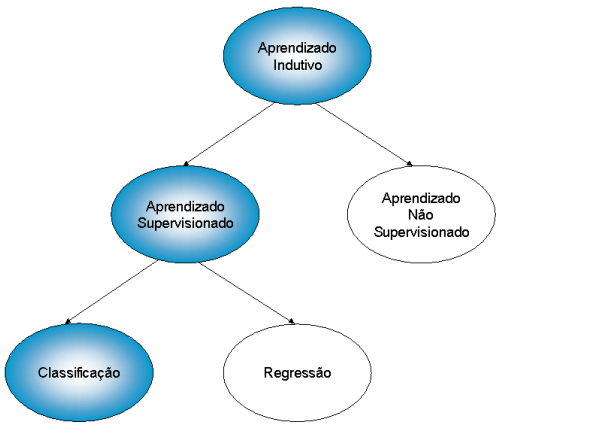
\includegraphics[width=15cm]{figuras/classificacao_regressao}}
		}{
		\Fonte{\cite{rezende_sistemas_2003}}			
	}	
\end{figure}

Por outro lado, em problemas de regressão, o valor a ser previsto é contínuo, pertencente a um domínio numérico não discreto. Casos típicos incluem a estimativa do valor de imóveis com base em suas características ou a previsão de temperatura a partir de dados meteorológicos. Nesses casos, o modelo busca aproximar os valores reais por meio de uma função inferida dos dados \cite{hastie_elements_2009}.

Além de sua aplicação em tarefas tradicionais de previsão, a regressão também serve de base conceitual para modelos generativos modernos, como os modelos de linguagem natural. Esses sistemas, fundamentados em arquiteturas de transformadores, são treinados para prever a próxima palavra (ou token) com base no contexto anterior, modelando distribuições condicionais sobre sequências de texto. Tarefas como language modeling (modelagem de linguagem) ou masked language modeling (modelagem de linguagem mascarada) são formuladas como problemas supervisionados em grandes corpora textuais, com pares entrada/saída derivados automaticamente \cite{devlin_bert:_2018}.

A aprendizagem supervisionada pressupõe uma relação entre os valores de entrada e suas respectivas saídas. Do ponto de vista matemático, essa abordagem pode ser formalizada da seguinte maneira: dado um conjunto de treinamento com \( N \) pares de entrada-saída

\[
(x_1, y_1), (x_2, y_2), \dots, (x_N, y_N),
\]

onde cada \( y_j \) foi gerado por uma função desconhecida \( f(x) \), o objetivo da aprendizagem é encontrar uma função \( h \), denominada hipótese, que se aproxime da verdadeira função \( f \). Assim, deseja-se que

\[
h(x) \approx f(x)
\]

para todos os exemplos, inclusive os ainda não vistos. Para medir a acurácia de uma hipótese, fornece-se a ela um conjunto de teste com exemplos distintos do conjunto de treinamento. Diz-se que uma hipótese generaliza bem se ela prediz corretamente o valor de \( y \) para exemplos novos. 

Às vezes, a função \( f \) é estocástica — ou seja, não é estritamente uma função de \( x \) — e, nesse caso, o que se deseja aprender é uma distribuição de probabilidade condicional, \( P(Y \mid x) \).

Em última instância, a aprendizagem supervisionada, como os demais paradigmas de aprendizado de máquina, contribui diretamente para o desenvolvimento de agentes inteligentes capazes de adaptar seu comportamento com base na experiência. Como sintetizado por \citeonline{russell_artificial_2016}, o cerne da Inteligência Artificial está em projetar sistemas que possam agir racionalmente, isto é, tomar decisões que maximizem suas chances de sucesso com base em informações disponíveis. O aprendizado, nesse contexto, emerge como mecanismo fundamental para equipar esses agentes com a capacidade de inferir, generalizar e se aprimorar continuamente diante de novos desafios.

Portanto, ao entender a aprendizagem como um processo sistemático de aproximação entre dados e conhecimento, por meio da inferência de padrões e relações estatísticas, reafirma-se sua posição como um dos pilares da Inteligência Artificial moderna. Essa perspectiva amplia o alcance dos sistemas computacionais para além de tarefas programadas explicitamente, permitindo que eles operem de forma mais autônoma, robusta e eficaz em ambientes complexos e dinâmicos.


\section{Redes Neurais Artificiais (RNA)}
\label{sec:redes-neurais-artificiais}

Como foi visto na seção anterior, o campo de estudo do Aprendizado de Máquina (AM) tem como principal objeto o processo de aprendizagem em si, buscando não apenas compreender como ela ocorre, mas também desenvolver métodos que permitam incorporar essa capacidade aos sistemas computacionais. Boa parte dos esforços desse campo se concentra em introduzir nos algoritmos a habilidade de melhorar seu desempenho com base na experiência passada, de forma semelhante ao que ocorre com seres humanos ao longo do tempo.

Entre as abordagens mais influentes no contexto do AM, destacam-se as Redes Neurais Artificiais (RNAs), cujo desenvolvimento foi fortemente influenciado pelas descobertas no campo da neurociência. Graças a pesquisadores como Camillo Golgi e Santiago Ramón y Cajal, tornou-se possível estudar a estrutura e o funcionamento dos neurônios, as unidades básicas do sistema nervoso. Essas células, ao se interconectarem em redes complexas, demonstram ser capazes de realizar tarefas cognitivas fundamentais, além de estarem na base da formação da consciência (SEARLE, 1992).

Na estrutura de uma rede neural biológica, os neurônios interagem entre si por meio de sinais, criando conexões chamadas sinapses. É através desse processo que estímulos externos são transformados em impulsos elétricos e químicos, que se propagam pela rede e ativam diferentes grupos de neurônios, cada um associado a funções específicas do sistema nervoso. Como resultado dessa ativação coordenada, o cérebro é capaz de gerar respostas complexas a partir de entradas sensoriais aparentemente simples \cite{kandel_principles_2013}.

A unidade básica de um neurônio é constituída pelo corpo da célula, ou soma, que contém o núcleo celular. Ramificando-se do corpo celular, encontramos numerosas fibras chamadas dendritos e uma única e longa fibra conhecida como axônio, como pode ser visto na Figura \ref{fig:neronicos_estrutura}. O axônio pode se estender por uma distância considerável — tipicamente 1 cm (100 vezes o diâmetro do corpo celular), mas pode chegar a até 1 metro de comprimento. Um neurônio pode fazer conexões com 10 a 100.000 outros neurônios nas junções sinápticas.

\begin{figure}[h!]
		\centering
		\Caption{\label{fig:neronicos_estrutura} Estrutura de um neurônio}	
		\UNIFORfig{}{
			\fbox{\includegraphics[width=15cm]{figuras/neurônio.png}}
		}{
		\Fonte{\cite{kandel_principles_2013}}			
	}	
\end{figure}


Os sinais são propagados de neurônio para neurônio por meio de uma complexa reação eletroquímica. Esses sinais controlam a atividade cerebral a curto prazo e também possibilitam mudanças de longo prazo na conectividade dos neurônios. Acredita-se que esses mecanismos formam a base do aprendizado no cérebro \cite{russell_artificial_2016}.

Com o avanço no estudo do funcionamento do cérebro humano e a descrição detalhada das redes biológicas que o compõem, foi possível para pioneiros como Warren McCulloch e Walter Pitts propor, em 1943, um modelo matemático de neurônio artificial. Seu trabalho introduziu um sistema lógico baseado em redes de unidades binárias interconectadas, onde cada unidade imitava de forma abstrata o comportamento de um neurônio biológico, como se pode ver na Figura \ref{fig:neuron_modelo}. Como sua contraparte biológica, o neurônio artificial emite um sinal de ativação em resposta ao estímulo que recebe \cite{mcculloch_logical_1943}.

\begin{figure}[h!]
		\centering
		\Caption{\label{fig:neuron_modelo} Estrutura de um neurônio}	
		\UNIFORfig{}{
			\fbox{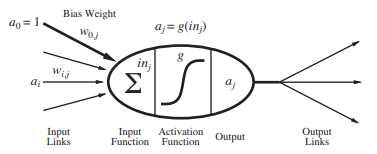
\includegraphics[width=15cm]{figuras/neuron_model.png}}
		}{
		\Fonte{\cite{russell_artificial_2016}}			
	}	
\end{figure}

O sinal é emitido quando o input recebido excede um limiar (threshold), que pode ser definido de forma rígida (hard threshold) ou flexível (soft threshold), dependendo do modelo adotado.

Esse comportamento é representado na modelagem através de uma função de ativação que recebe o resultado da combinação linear entre os pesos sinápticos e as respectivas componentes do input. Essa combinação pode ser expressa por:

\[
y = f\left(\sum_{i=1}^{n} w_i x_i + b\right)
\]

onde \(x_i\) representa as entradas do neurônio, \(w_i\) os pesos associados a cada entrada, \(b\) o termo de viés \textit{bias} e \(f\) a função de ativação. Essa função tem o papel de introduzir não-linearidade no modelo, sendo essencial para que a rede neural artificial seja capaz de aprender relações complexas entre os dados de entrada.

Um dos modelos mais básicos de neurônio artificial é o perceptron, introduzido por \cite{rosenblatt_perceptron:_1958}. O perceptron é caracterizado pelo uso de uma função de ativação do tipo limiar rígido (hard threshold), que emite uma saída binária dependendo se a soma ponderada das entradas ultrapassa ou não um determinado limiar. Dessa forma, a unidade produz um sinal “ligado” ou “desligado”, similar a um interruptor.

Partindo do perceptron isolado, as redes neurais são formadas pela conexão de múltiplas unidades, organizadas em camadas. Uma das diferentes formas de agrupar essas estruturas é a arquitetura MLP (Multilayer Perceptron), que possui conexões apenas unidirecionais --- ou seja --- forma um grafo direto e acíclico.

Nessa arquitetura, as unidades são organizadas em camadas distintas: a camada de entrada, uma ou mais camadas ocultas e a camada de saída (Figura \ref{fig:hiden_layer}). Cada neurônio de uma camada está conectado a neurônios da próxima camada, propagando a ativação de forma sequencial, sem ciclos de retorno.

\begin{figure}[h!]
		\centering
		\Caption{\label{fig:hiden_layer} Rede Neural pós aprendizado}	
		\UNIFORfig{}{
			\fbox{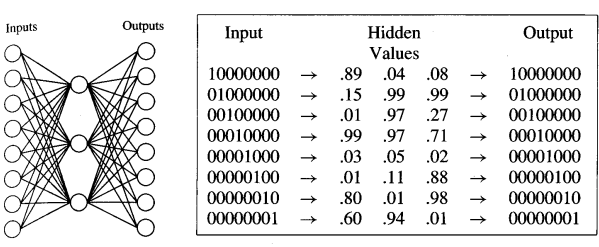
\includegraphics[width=15cm]{figuras/rede_neural_hiden_layer.png}}
		}{
		\Fonte{\cite{mitchell_machine_2013}}			
	}	
\end{figure}

 Cada neurônio opera calculando uma combinação ponderada das ativações recebidas da camada anterior. Sobre essa soma ponderada, é aplicada uma função de ativação não linear, que introduz complexidade e permite à rede modelar relações não-lineares nos dados. O resultado dessa operação é então transmitido como entrada para os neurônios da próxima camada \cite{russell_artificial_2016}. Essa estrutura hierárquica, composta por múltiplas camadas, possibilita que a rede construa representações progressivamente mais abstratas e complexas dos dados à medida que os sinais fluem através dela. Cada camada aprende a extrair características de um nível diferente de abstração, passando informações mais refinadas para a camada subsequente \cite{goodfellow_deep_2016}.

A ausência de ciclos simplifica o processo de treinamento e torna possível o uso do algoritmo de retropropagação para ajustar os pesos sinápticos. Este algoritmo é a espinha dorsal do aprendizado na maioria das redes neurais, pois permite ajustar os pesos sinápticos dos neurônios de forma a minimizar o erro entre a saída prevista pela rede e a saída desejada (o valor real ou o rótulo correto) \cite{rumelhart_learning_1986}. 

O aprendizado efetivamente ocorre com o ajuste iterativo dos pesos em cada neurônio, em cada camada da rede. O processo começa com a propagação forward: os dados de entrada ativam a camada inicial e são processados sequencialmente através das camadas ocultas até atingirem a camada de saída, onde a rede gera uma predição. Em seguida, a etapa de retropropagação se inicia. O erro entre a predição da rede e o valor esperado é calculado e, a partir daí, é propagado no sentido inverso, da camada de saída de volta para as camadas de entrada. Durante essa propagação reversa, os pesos de cada conexão são atualizados de forma a reduzir gradualmente esse erro nas iterações futuras. É esse ciclo contínuo de propagação forward e retropropagação que permite à rede "aprender" a partir dos dados.

Assim, uma das principais características de uma rede neural é sua intrínseca capacidade de aprender, ou seja, sua habilidade de se aproximar e modelar funções complexas. A quantidade e a complexidade das funções que podem ser representadas por essa arquitetura dependem diretamente do número de camadas (profundidade da rede) e da quantidade de neurônios em cada uma delas, o que permite que redes neurais, especialmente as profundas, aprendam representações incrivelmente sofisticadas e não-lineares dos dados \cite{mitchell_machine_2013}.

\section{Aprendizado Profundo}
\label{sec:aprendizado-de-maquina}

De acordo com o Paradoxo de Morovac, articulado na obra Mind Child por \citeonline{moravec_mind_1995}, tarefas que envolvem raciocínio lógico complexo, muitas vezes difíceis para seres humanos, são relativamente fáceis para sistemas computacionais, enquanto for possível uma descrição clara da tarefa. Exemplos claros incluem o fato de que jogar xadrez em nível de grande mestre ou resolver equações matemáticas avançadas são comparativamente simples de programar para computadores. No entanto, localizar objetos em uma imagem, compreender a fala em um ambiente ruidoso e manipular objetos na vida real, tarefas realizadas instintivamente por humanos e difíceis de descrever através de parâmetros, mostraram-se extraordinariamente difíceis de replicar em máquinas.

É nesse contexto que redes neurais artificiais, como apresentado na sessão anterior, emergem como uma abordagem promissora. A hipótese central por trás das redes neurais é que qualquer problema complexo pode ser aproximado por uma função matemática. Dada uma quantidade suficientemente grande de dados de treinamento e uma arquitetura adequada, redes neurais com múltiplas camadas ocultas (as chamadas redes "profundas") demonstram uma notável capacidade de aprender e se aproximar de funções de ordem extremamente complexa. Esta propriedade fundamental é formalizada pelo Teorema da Aproximação Universal \cite{hornik_multilayer_1989}.

A capacidade de representação dessas redes profundas provém justamente da presença de múltiplas camadas ocultas, que possibilitam a extração de padrões e abstrações em diferentes níveis de complexidade. No entanto, apesar do seu potencial teórico, durante muitos anos o treinamento eficaz dessas redes permaneceu um desafio, principalmente pela dificuldade em ajustar os pesos das camadas intermediárias de forma eficiente.

Somente a partir de 1986, com a publicação pelo autor \citeonline{rumelhart_learning_1986} do artigo "Learning Internal Representations by Error Propagation", esse obstáculo pode ser superado. Nesse trabalho, foi apresentado o algoritmo de retropropagação do erro (backpropagation), que tornou viável o treinamento de redes com múltiplas camadas. A técnica baseia-se no uso do gradiente do erro para atualizar os pesos da rede, propagando esse gradiente da camada de saída para as camadas anteriores.

Esse algoritmo é dividido em dois processos complementares: a propagação direta (forward propagation) e a retropropagação do erro (backward propagation). Na primeira etapa, os dados de entrada percorrem a rede camada por camada, sendo transformados por combinações lineares seguidas da aplicação de funções de ativação não lineares, até a obtenção da saída final. Em seguida, calcula-se o erro, que corresponde à diferença entre a saída obtida e a saída esperada.

Na segunda etapa, esse erro é propagado de volta pelas camadas da rede, utilizando o método do gradiente descendente para ajustar os pesos de forma a minimizar uma função de custo. Essa atualização ocorre iterativamente, permitindo que a rede aprenda a partir dos exemplos apresentados. Com o tempo, a rede se ajusta para realizar previsões mais precisas.

Apesar do avanço fundamental proporcionado pelo algoritmo de retropropagação, o potencial total das redes neurais profundas permaneceu, por muito tempo, inexplorado. Foi somente em 2012, com o sucesso da arquitetura AlexNet no desafio ImageNet \cite{krizhevsky_imagenet_2017}, que o aprendizado profundo passou a ganhar notoriedade. A partir desse avanço, diversos fatores convergiram para alavancar o desenvolvimento dessa área.

De acordo com \citeonline{lecun_deep_2015}, três fatores principais foram determinantes para essa ascensão:

\begin{itemize}
    \item \textbf{Uso Eficiente de GPUs:} A capacidade de processar grandes volumes de dados em paralelo, utilizando unidades de processamento gráfico (GPUs), tornou o treinamento de modelos profundos computacionalmente viável e rápido.

    \item \textbf{Inovações Algorítmicas:} A adoção de funções de ativação mais eficientes, como as Retified Linear Units (ReLUs), que ajudaram a mitigar problemas de gradiente em redes profundas, e o desenvolvimento de novas técnicas de regularização, como o Dropout, que previne o overfitting, foram cruciais.

    \item \textbf{Aumento de Dados:} A capacidade de gerar mais exemplos de treinamento através de técnicas de aumento de dados (data augmentation), que deformam os dados existentes (como rotações, cortes e espelhamentos de imagens), expandiu significativamente os conjuntos de dados disponíveis e melhorou a generalização dos modelos.
\end{itemize}

A partir desses avanços combinados, a aprendizagem profunda não apenas superou as limitações históricas do aprendizado de máquina, mas também impulsionou um salto qualitativo na capacidade da IA de lidar com tarefas de percepção complexas, como visão computacional, reconhecimento de voz e recomendação de conteúdos.

Um dos campos mais impactados por essa evolução foi o Processamento de Linguagem Natural (PLN), que até então enfrentava grandes obstáculos na modelagem de estruturas linguísticas altamente variáveis e ambíguas. Inicialmente, o uso de Redes Neurais Recorrentes (RNNs) e suas variantes, como as LSTMs (Long Short-Term Memory) \cite{hochreiter_long_1997}, marcou um avanço importante na modelagem sequencial de texto, permitindo que padrões temporais e dependências de longo prazo fossem aprendidos diretamente a partir de grandes volumes de dados linguísticos. No entanto, mesmo com as melhorias, as RNNs e LSTMs possuíam limitações intrínsecas, principalmente relacionadas à dificuldade de capturar dependências de longo prazo em sequências muito extensas e à dificuldade de paralelização de seu treinamento em larga escala.

Como veremos mais adiante, uma arquitetura inovadora surgiria para transformar o campo do PLN mais uma vez, superando essas barreiras e pavimentando o caminho para os modelos de linguagem que conhecemos hoje.

\section{Processamento de Linguagem Natural}
\label{sec:processamento-de-linguagem-natural}

A linguagem, tanto escrita quanto falada, é um dos diversos atributos que distingue o Homo sapiens de todas as outras espécies que andam, voam, nadam ou rastejam na superfície da terra. Por volta de 100.000 anos atrás, humanos aprenderam a falar, e por volta de 7.000 anos atrás, a escrever. Apesar de haver espécies capazes de demonstrar vocabulário de centenas de sinais, apenas humanos foram capazes de desenvolver e usar linguagens para comunicar um número indeterminado de mensagens e ideias \cite{russell_artificial_2016}.

Linguagens formais, como as de programação (Java e Python), possuem regras e uma semântica rígida que delimitam um número infinito de programas válidos, chamados de gramática. Essas linguagens são incorporadas nos sistemas computacionais e podem ter seu "sentido" interpretado e traduzido diretamente para a linguagem nativa das máquinas. No entanto, as linguagens naturais, como Português e Inglês, são intrinsecamente mais complexas e ambíguas. Elas não seguem um conjunto de regras fixas e facilmente formalizáveis; em vez disso, evoluem organicamente e dependem fortemente do contexto, da cultura, das nuances de entonação e da intenção do falante para que seu significado seja plenamente compreendido \cite{jurafsky_speech_2009}. A mesma palavra pode ter múltiplos significados, e a estrutura de uma frase pode variar enormemente sem alterar seu sentido essencial, tornando a interpretação computacional um desafio substancial.

Assim, para que a tarefa de análise de linguagem natural seja feita por máquinas, além de compreender os símbolos que compõem a língua, é preciso que seu sentido seja descrito de forma clara e sem ambiguidade, através de regras e padrões, para o sistema computacional, de modo que seu significado possa ser devidamente capturado — algo próximo do que é feito com as linguagens formais. Nesse sentido, podemos entender o PLN como uma área interdisciplinar que reúne conhecimentos da Ciência da Computação, Inteligência Artificial e Linguística. Seu objetivo é desenvolver métodos e algoritmos que permitam às máquinas não apenas processar o texto ou a fala, mas também compreender as intenções e o significado por trás da comunicação humana

Historicamente, as primeiras tentativas de fazer computadores entenderem a linguagem foram fundamentadas em regras gramaticais explícitas, elaboradas programaticamente e inseridas a mão nos sistemas responsáveis pelo processamento. No entanto, a natureza ambígua e irrestrita inerente à linguagem natural, além das inflexões que toda linguagem sofre quando usadas de fato, revelaram a impraticabilidade dessa abordagem puramente simbólica e artesanal \cite{nadkarni_natural_2011}.

Processamento de Linguagem natural deve extrair o sentido (semântica) do texto, assim, um dos principais desafios enfrentados era: As gramáticas formais especificam principalmente a sintaxe (a relação entre unidades de texto, como substantivos, verbos e adjetivos). Embora fosse possível estender essas gramáticas para abordar a semântica da linguagem natural através da expansão massiva de subcategorias e regras adicionais (por exemplo, a regra de que o verbo "comer" se aplica apenas a substantivos de itens ingeríveis) \cite{nadkarni_natural_2011}, isso levava a dois problemas críticos:

\begin{enumerate}
    \item \textbf{Explosão de Regras e Interações Imprevisíveis:} As regras tornavam-se incontrolavelmente numerosas e, muitas vezes, interagiam de maneira imprevisível, levando a um aumento na frequência de "interpretações ambíguas" (múltiplas interpretações possíveis para uma sequência de palavras). Exemplos como trocadilhos (ambiguidades usadas para efeito humorístico) demonstram a sutileza com que humanos lidam com a polissemia, algo que sistemas baseados em regras falhavam.
    \item \textbf{Inflexibilidade com Variações Linguísticas:} Regras escritas à mão lidavam muito mal com a prosa não-gramatical da fala cotidiana e com textos altamente telegráficos (como notas de progresso hospitalares em contextos médicos), que, embora compreendidos por humanos, desviavam-se das estruturas formais esperadas.
\end{enumerate}

Essas limitações impulsionaram o surgimento do PLN Estatístico no final do século XX. Essa nova abordagem focava em aprender padrões a partir de grandes corpora de texto, utilizando modelos probabilísticos e técnicas de aprendizado de máquina. Em vez de regras explícitas, os sistemas estatísticos inferiam as probabilidades de ocorrência de palavras e sequências, permitindo uma maior robustez à variabilidade e ambiguidade da linguagem real.

Uma das grandes sacadas das últimas cinco décadas de pesquisa em processamento de linguagem é que o vasto e complexo conhecimento linguístico pode ser capturado por um número limitado de modelos formais e teorias. Felizmente, esses modelos são derivados de ferramentas padrão da ciência da computação, matemática e linguística \cite{jurafsky_speech_2009}. Entre os mais importantes estão:

\begin{itemize}
    \item \textbf{Máquinas de Estado:} Em sua formulação mais simples, são modelos formais que consistem em estados, transições entre estados e uma representação de entrada. Variações comuns incluem autômatos finitos determinísticos e não determinísticos, e transdutores de estados finitos. Esses modelos são cruciais para lidar com o conhecimento de fonologia, morfologia e sintaxe, frequentemente complementados por sistemas de regras formais, como gramáticas regulares e livres de contexto.
    \item \textbf{Lógica:} Modelos baseados em lógica, como a lógica de primeira ordem (cálculo de predicados), têm sido tradicionalmente empregados para modelar a semântica e a pragmática da linguagem. Eles visam representar o significado e as relações lógicas dentro de sentenças, embora abordagens mais recentes tenham se voltado para técnicas mais robustas da semântica lexical não-lógica.
    \item \textbf{Modelos Probabilísticos:} Cruciais para capturar todo tipo de conhecimento linguístico, esses modelos permitem que cada uma das abordagens anteriores (máquinas de estado, sistemas de regras e lógica) seja aumentada com probabilidades. Por exemplo, uma máquina de estado pode se tornar um autômato ponderado ou um Modelo de Markov. Dentre eles, os Modelos de Markov Ocultos (\textit{HMMs - Hidden Markov Models}) foram amplamente utilizados em diversas aplicações do PLN, como marcação de classes gramaticais \textit{(part-of-speech tagging}), reconhecimento de fala, compreensão de diálogo e tradução automática. A principal vantagem dos modelos probabilísticos é sua capacidade de resolver os diversos problemas de ambiguidade; quase qualquer problema de processamento de fala e linguagem pode ser reformulado como: "dadas N escolhas para alguma entrada ambígua, escolha a mais provável" \cite{jurafsky_speech_2009}.

    \item \textbf{Modelos de Espaço Vetorial:} Baseados em álgebra linear, esses modelos são a base da recuperação de informação e de muitos tratamentos do significado das palavras, onde palavras e documentos são representados como vetores numéricos em um espaço multidimensional. A proximidade entre vetores indica similaridade semântica.
\end{itemize}

No entanto, os avanços recentes no campo do aprendizado profundo provocaram uma verdadeira revolução na forma como os sistemas computacionais compreendem e geram linguagem natural. Enquanto os modelos estatísticos clássicos dependiam significativamente de engenharia de características — ou seja, da extração manual de atributos linguísticos relevantes para alimentar os modelos —, as redes neurais profundas trouxeram a capacidade de aprender automaticamente essas representações diretamente a partir dos dados brutos \cite{lecun_deep_2015, goodfellow_deep_2016}. Essa abordagem tornou possível capturar padrões complexos e hierarquias de significado que antes eram inacessíveis ou exigiam considerável intervenção humana.

Dentre os principais marcos dessa transformação, destacam-se os modelos baseados em Redes Neurais Recorrentes (RNNs), especialmente suas variantes mais sofisticadas, como as LSTMs (Long Short-Term Memory) \cite{hochreiter_long_1997} e as GRUs (Gated Recurrent Units). Essas arquiteturas foram desenvolvidas para lidar com dados sequenciais e se mostraram eficazes ao modelar dependências temporais e contextuais, superando muitas limitações dos modelos probabilísticos tradicionais. Elas obtiveram destaque em diversas tarefas de Processamento de Linguagem Natural, como tradução automática, sumarização, classificação de sentimentos e resposta a perguntas.

Apesar dos avanços, as RNRs ainda apresentavam limitações estruturais importantes. Por dependerem de um processamento estritamente sequencial — palavra por palavra —, essas redes impunham restrições significativas à paralelização durante o treinamento, além de apresentarem dificuldades em capturar relações de longa distância dentro dos textos. Esses desafios se tornaram ainda mais críticos com o aumento exponencial do volume de dados e da complexidade das tarefas linguísticas modernas.

Foi nesse contexto de crescente demanda por modelos mais eficientes e expressivos que emergiu uma nova classe de arquiteturas que dispensam a recorrência e introduzem mecanismos mais flexíveis de processamento sequencial. A próxima seção explora em detalhe esse novo paradigma que redefiniu o estado da arte no PLN contemporâneo: a Arquitetura Transformer \cite{vaswani_attention_2017}.


\section{Arquitetura Transformer}
\label{sec:arquitetura-transformer}

Como discutimos na seção anterior, o campo de Processamento de Linguagem Natural (PLN) teve avanços significativos com o surgimento do aprendizado profundo. Tarefas clássicas da área, como análise de sentimentos, reconhecimento de entidades nomeadas e tradução automática, passaram a ser tratadas com redes neurais, especialmente as recorrentes \cite{ansar_survey_2024}. Contudo, essas arquiteturas enfrentavam desafios consideráveis, como a dificuldade de capturar dependências de longo prazo em sequências muito extensas e a ineficiência no treinamento em larga escala devido à sua natureza sequencial. O verdadeiro divisor de águas no desempenho desses sistemas, que superou essas limitações e redefiniu o campo, foi a introdução da arquitetura conhecida como \textit{Transformer}.

Proposta em 2017 por Vaswani e colaboradores, no artigo seminal \textit{Attention Is All You Need} \cite{vaswani_attention_2017}, a arquitetura Transformer revolucionou a forma como os modelos processam sequências de linguagem. Ela se tornou a base para o desenvolvimento de modelos amplamente utilizados atualmente, como o \textit{Bidirectional Encoder Representations from Transformers} (BERT) e os \textit{Generative Pre-trained Transformers} (GPT) \cite{topal_exploring_2021}.

O principal diferencial do \textit{Transformer} está no uso intensivo do mecanismo de atenção, que permite ao modelo avaliar a importância relativa de cada palavra no contexto de uma sentença. Isso possibilita a codificação de relações complexas entre palavras, mesmo quando estão distantes entre si na sequência textual. Ao contrário das redes recorrentes, que processam a entrada de forma sequencial, essa nova arquitetura
opera de forma paralela, o que o torna substancialmente mais eficiente para tarefas de treinamento em larga escala \cite{vaswani_attention_2017}.

Para compreender plenamente o impacto dessa abordagem e como o \textit{Transformer} avalia a significância das palavras, é necessário primeiro entender o processo fundamental de codificação de palavras e como essa representação evoluiu das arquiteturas anteriores. Durante os anos 2000, como uma maneira de suprir a incapacidade dos modelos de linguagem estatísticos tradicionais em lidar com a relação semântica entre conceitos e o contexto da linguagem, foi desenvolvida a técnica de \textit{embedding} \cite{ansar_survey_2024}.

A técnica de \textit{word embedding} consiste em representar uma palavra num espaço vetorial contínuo de alta dimensionalidade. Nesses espaços, palavras com significados semelhantes ou que ocorrem em contextos parecidos são mapeadas para vetores numericamente próximos. Essa proximidade vetorial captura relações semânticas e sintáticas, permitindo que os modelos de PLN interpretem o "sentido" das palavras de uma forma que as abordagens simbólicas ou \textit{one-hot} não conseguiam.

Modelos como Word2Vec \cite{mikolov_distributed_2013} e GloVe \cite{pennington_glove:_2014} tornaram-se fundamentais nesse processo, permitindo a captura de relações léxicas e semânticas de maneira eficiente. Ao invés de tratar cada palavra como uma entidade discreta, como nos métodos de representação \textit{one-hot} (onde cada palavra no vocabulário recebia um vetor binário com um "1" na posição correspondente e "0" nas demais, resultando em vetores esparsos sem relações semânticas intrínsecas), os \textit{embeddings} incorporaram informação contextual distribuída, extraída de grandes corpora de texto. Essa mudança permitiu que os modelos compreendessem, por exemplo, que "rei" e "rainha" estão relacionados por um padrão vetorial semelhante ao de "homem" e "mulher", tornando as representações mais ricas e significativas para o processamento computacional da linguagem.

A representação numérica de palavras por meio de embeddings não apenas ampliou a capacidade das máquinas de capturar nuances semânticas, como também reduziu significativamente o custo computacional, ao projetar essas palavras em um espaço vetorial mais compacto e denso. Modelos especializados na geração desses embeddings passaram a ser amplamente integrados a arquiteturas do tipo Encoder-Decoder, especialmente aquelas baseadas em Redes Neurais Recorrentes (RNNs) e em suas variantes mais sofisticadas, como as LSTMs e GRUs. Nesses modelos, o encoder processa a sequência de entrada palavra por palavra, transformando os embeddings em um vetor de contexto que resume as informações relevantes da sentença \cite{fu_decoder-only_2023}.

A estrutura Encoder-Decoder constitui a base da maioria dos modelos neurais de transdução de sequência mais competitivos \cite{vaswani_attention_2017}. Nessa arquitetura, o encoder recebe como entrada uma sequência de representações simbólicas
$(x_1, x_2, \ldots, x_n)$
e a transforma em uma sequência de representações contínuas
$\mathbf{z} = (z_1, z_2, \ldots, z_n)$,
as quais servem como base para a etapa de decodificação realizada pelo decoder.

A arquitetura Transformer adota essa estrutura geral, substituindo a recorrência por mecanismos de autoatenção empilhados e camadas totalmente conectadas (fully connected, aplicadas ponto a ponto), tanto no encoder quanto no decoder, como ilustrado nas metades esquerda e direita da Figura~\ref{fig:trasnformers_arquitetura}, respectivamente.

\begin{figure}[h!]
		\centering
		\Caption{\label{fig:trasnformers_arquitetura} Arquitetura Transformers}	
		\UNIFORfig{}{
			\fbox{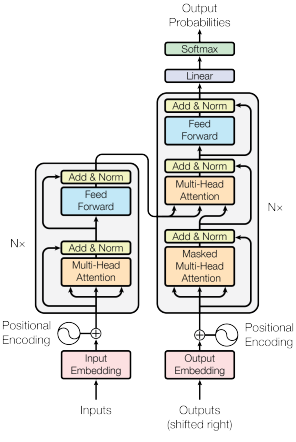
\includegraphics[width=9cm]{figuras/trasnformers_arquitetura.png}}
		}{
		\Fonte{\cite{vaswani_attention_2017}}			
	}	
\end{figure}

Como já foi dito, o sistema de atenção particular dessa arquitetura é o que faz ela se destacar. Tal sistema é nomeado como \textit{Scaled Dot-Product Attention}. 

Sistemas de atenção, em geral, funcionam como um mapeamento entre uma \textit{querie} e um conjunto de pares chave-valor \textit{(key-value)} para uma saída. Nessa formulação, a \textit{querie}, a chave, o valor e a saída são todos vetores. A saída é calculada como uma soma ponderada dos valores, onde o peso atribuído a cada valor é computado por uma função de compatibilidade entre a \textit{querie} e a chave correspondente. Este conceito permite que o modelo foque dinamicamente nas partes mais relevantes da entrada ao gerar uma saída, em vez de tratar todos os elementos da mesma forma \cite{vaswani_attention_2017}.

\begin{figure}[h!]
    \centering
    \Caption{\label{fig:scald_dot_multi_head} (Esquerda) Atenção escalada por produto escalar e (direita) atenção multi-cabeça .}  
    \UNIFORfig{}{
        \fbox{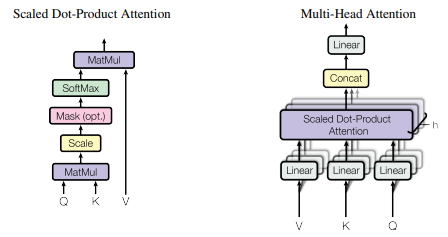
\includegraphics[width=12cm]{figuras/scald_dot_multi_head.png}}
    }{
        \Fonte{\cite{vaswani_attention_2017}}         
    }   
\end{figure}


Especificamente no Transformer, a atenção é implementada como atenção escalada por produto escalar, ou \textit{Scaled Dot-Product Attention} (Figura \ref{fig:scald_dot_multi_head}). Dado um conjunto de \textit{querie} $Q$, chaves $K$ e valores $V$, todos de dimensão $d_k$, computa-se o produto escalar entre as \textit{queries} e todas as chaves, divide-se por $\sqrt{d_k}$ para estabilizar os gradientes, e aplica-se uma função \textit{softmax} para obter os pesos de atenção. Em seguida, esses pesos são utilizados para calcular uma média ponderada dos valores. A operação completa é expressa da seguinte forma:

\begin{equation}
\text{Attention}(Q, K, V) = \text{softmax} \left( \frac{QK^\top}{\sqrt{d_k}} \right) V
\end{equation}

Essa forma se aproxima da função de atenção por produto escalar, mas com um ajuste: o fator de escalonamento \( \frac{1}{\sqrt{d_k}} \). Na ausência desse fator, quando comparada à função de atenção aditiva, para valores grandes de \( d_k \), os produtos escalares entre as \textit{queries} e as \textit{keys} tendem a assumir valores de grande magnitude. Isso faz com que os resultados da função \textit{softmax} se aproximem de uma distribuição esparsamente concentrada (quase \textit{one-hot}), o que leva a gradientes extremamente pequenos durante a retropropagação. Como consequência, o aprendizado do modelo se torna ineficiente ou até instável \cite{vaswani_attention_2017}.

Para ampliar ainda mais a capacidade do modelo de capturar diferentes tipos de relacionamentos entre palavras, o \textit{Transformer} utiliza um mecanismo chamado \textit{Multi-Head Attention}. Em vez de calcular uma única atenção, o modelo executa várias operações de atenção em paralelo, cada uma com diferentes projeções lineares de $Q$, $K$ e $V$. Os resultados dessas diferentes "cabeças" são então concatenados e projetados novamente, permitindo que o modelo aprenda múltiplas representações contextuais de diferentes subespaços de atenção de forma simultânea.

Esse mecanismo não apenas enriquece a representação contextual de cada palavra na sequência, como também favorece a modelagem de dependências complexas — algo essencial para tarefas como tradução, sumarização e geração de texto.

Com essa fundação, o \textit{Transformer } se estabelece como uma arquitetura altamente paralelizável, estável durante o treinamento e eficaz em capturar estruturas linguísticas profundas. Esses fatores explicam seu sucesso generalizado em modelos de linguagem de larga escala, como BERT e GPT.

\section{Modelos de Linguagem de Grande Escala (LLMs)}
\label{sec:modelos-de-linguagem-de-grande-escala}

O advento da arquitetura Transformer possibilitou o treinamento em paralelo de modelos de linguagem, graças ao seu mecanismo de atenção baseado em produto escalar. Além disso, essa arquitetura abordou desafios clássicos relacionados à perda ou explosão do gradiente — problemas recorrentes em redes profundas — ao empregar uma função de ativação como a \textit{softmax} combinada com um fator de escalonamento. Essa solução permitiu que os modelos processassem e aprendessem efetivamente com sequências de texto muito mais longas durante o treinamento, superando uma das principais limitações das arquiteturas anteriores \cite{vaswani_attention_2017}.

Com esse avanço, surgiram os chamados Modelos de Linguagem de Grande Escala, ou Large Language Models (LLMs), que se tornaram o novo paradigma no campo do Processamento de Linguagem Natural (PLN). Os LLMs são modelos estatísticos de linguagem baseados em redes neurais, treinados em larga escala com quantidades massivas de dados textuais. Seu sucesso recente é fruto de décadas de pesquisa e desenvolvimento em modelagem de linguagem, combinando inovações arquiteturais com avanços significativos em capacidade computacional e disponibilidade de dados \cite{wu_multimodal_2023, brown_language_2020}.

Esses modelos possuem a capacidade de generalizar para uma ampla variedade de tarefas linguísticas com pouco ou nenhum ajuste adicional, o que revolucionou o modo como interagimos com sistemas computacionais baseados em linguagem. Quando comparados aos seus predecessores, por exemplo, os Modelos de Linguagem Estatísticos (SLMs), possuem uma capacidade de generalização muito maior, removendo por inteiro a necessidade de arquiteturas especialistas em tarefas. 

Os LLMs mantêm uma estreita relação conceitual com os Modelos de Linguagem Pré-treinados (PLMs), pois ambos seguem o mesmo paradigma de treinamento em duas fases: pré-treinamento e fine-tuning. Nessa abordagem, modelos de linguagem, implementados em arquiteturas Transformer, são inicialmente pré-treinados em datasets gigantescos, compostos por texto não rotulado de escala web. O objetivo dessa fase é capacitar o modelo para tarefas genéricas, como a previsão da próxima palavra em uma sequência ou o preenchimento de lacunas em frases permitindo-lhe aprender um vasto conhecimento linguístico e factual, além de padrões complexos de gramática e semântica \cite{devlin_bert:_2018}.

Posteriormente, o modelo pré-treinado é ajustado (fine-tuned) para tarefas específicas, adaptando seu conhecimento geral a domínios ou requisitos particulares por meio de um treinamento com dados rotulados mais direcionados \cite{xu_contrastive_2024}.

No entanto, a grande diferença entre os PLMs menores e os LLMs reside fundamentalmente na escala massiva de parâmetros e dados de treinamento dos LLMs, combinada com a eficiência intrínseca da arquitetura Transformer. Essa capacidade de consumir e aprender com volumes sem precedentes de dados se apoia diretamente no paradigma de aprendizado auto-supervisionado.

O treinamento de modelos em uma escala de bilhões ou trilhões de tokens de texto, como é comum para LLMs, seria inviável com abordagens de aprendizado supervisionado tradicional, que exigem que humanos rotulem explicitamente cada exemplo de treinamento. Assim, o aprendizado auto-supervisionado, vem como uma forma de superar essa dificuldade, eliminando a dependência de datasets com dados rotulados. Invés disso, com acesso a uma fonte de dados brutos de escala adequada, sua rtulação é feita automaticamente \cite{balestriero_cookbook_2023}.

Assim, a disponibilidade massiva de dados e aprendizado semi-autonomo promoveram a captura profunda e ampla de padrões linguísticos e de conhecimento de mundo sem precedentes. Diferentemente dos PLMs menores ou dos modelos baseados em RNNs, cuja generalização era mais limitada e frequentemente exigia fine-tuning extensivo para cada nova tarefa, os LLMs exibem capacidades notáveis de aprendizado zero-shot e few-shot. Essas são consideradas habilidades emergentes, pois não são programadas diretamente, mas surgem de forma não linear à medida que a escala do modelo e dos dados de treinamento aumenta \cite{wei_emergent_2022}.

\begin{itemize}
    \item \textbf{Aprendizado \textit{Zero-Shot} \textit{(Zero-Shot Learning)}}: Esta capacidade permite que um LLM execute uma tarefa para a qual não foi explicitamente treinado, nem viu nenhum exemplo durante o pré-treinamento ou fine-tuning. O modelo consegue entender a instrução (dada em linguagem natural) e gerar uma resposta apropriada, confiando unicamente no vasto conhecimento e nas representações aprendidas durante sua fase de pré-treinamento massivo \cite{brown_language_2020}. Por exemplo, um LLM pode resumir um texto ou gerar um código em uma linguagem específica apenas com base na instrução, sem ter sido treinado em exemplos diretos dessa tarefa. 
    \item \textbf{Aprenizado \textit{Few-Shot} \textbf{(Few-Shot Learning)}}:  Nesta modalidade, o LLM é capaz de aprender a realizar uma nova tarefa com base em apenas um pequeno número de exemplos (tipicamente de 1 a 5). Ao observar esses poucos exemplos fornecidos no prompt (a instrução de entrada), o modelo infere o padrão ou a intenção da tarefa e aplica esse entendimento a novas entradas. Essa capacidade reduz drasticamente a necessidade de grandes datasets rotulados para fine-tuning em muitas aplicações, acelerando o desenvolvimento e a implantação \cite{brown_language_2020}.
\end{itemize}

Essas capacidades emergentes decorrem diretamente da diversidade e escala dos dados de pré-treinamento, combinadas à flexibilidade da arquitetura Transformer. O mecanismo de autoatenção permite a construção de representações contextuais ricas e eficientes, possibilitando que os modelos desenvolvam uma forma de "raciocínio implícito", frequentemente comparado a um senso comum artificial. Isso representa um avanço expressivo no processamento de linguagem natural e na interação entre humanos e máquinas.

No entanto, à medida que a escala desses modelos aumenta, surgem novos desafios relacionados à infraestrutura necessária para sua execução. Modelos como o GPT-3, LLaMA 3, Gemini e Copilot contam com bilhões de parâmetros, o que demanda uma capacidade computacional significativa tanto para o treinamento quanto para a inferência. Executá-los de maneira eficiente, especialmente em tempo real ou em dispositivos locais, requer soluções especializadas.

Para lidar com essas limitações, diversas estratégias têm sido desenvolvidas. Entre elas, destaca-se a quantização, uma técnica que reduz a precisão dos parâmetros do modelo (por exemplo, de 32 para 8 bits), diminuindo o consumo de memória e acelerando o tempo de inferência, com impacto mínimo na performance \cite{ansar_survey_2024}.  Outras técnicas incluem a poda (pruning), que remove conexões ou neurônios menos importantes, e a destilação de conhecimento (knowledge distillation), que treina um modelo menor para imitar o comportamento de um modelo maior.

Nesse contexto, plataformas como o Ollama surgiram como ferramentas cruciais para democratizar o acesso e o uso eficiente de LLMs. O Ollama permite aos usuários baixar e executar modelos de linguagem de grande escala (incluindo versões quantizadas de modelos populares como Llama 3, Mixtral e Gemma) diretamente em suas máquinas locais, aproveitando ao máximo o hardware disponível. Isso remove a dependência de infraestruturas de nuvem complexas e caras para inferência, facilitando o desenvolvimento de aplicações e a experimentação com LLMs em ambientes privados e controlados. Ao otimizar a execução para CPUs e GPUs de consumidor e ao suportar modelos em formatos mais eficientes, o Ollama exemplifica como as inovações em software e as técnicas de otimização tornam os LLMs mais acessíveis e aplicáveis em uma gama mais ampla de cenários.
\section{Ollama}

\label{sec:ollama}



Apesar do avanço sem precedentes dos Modelos de Linguagem de Grande Escala (LLMs) em capacidade e versatilidade, a execução desses modelos, especialmente em ambientes de desenvolvimento e produção, ainda apresenta desafios significativos. Modelos com bilhões ou trilhões de parâmetros, como GPT-3, LLaMA 3 e Gemini, demandam uma capacidade computacional e de memória substancial tanto para o treinamento quanto para a inferência. Executá-los de maneira eficiente, em tempo real ou em dispositivos locais, requer soluções que otimizem o uso dos recursos de hardware disponíveis \cite{ansar_survey_2024}.



Para lidar com essas limitações, diversas estratégias de otimização de modelos têm sido desenvolvidas. Entre as mais proeminentes, destaca-se a quantização, uma técnica que reduz a precisão numérica dos parâmetros do modelo (por exemplo, de 32 bits de ponto flutuante para 8 bits inteiros). Essa redução diminui drasticamente o consumo de memória e acelera o tempo de inferência, com um impacto frequentemente mínimo na performance e na acurácia do modelo final. Outras técnicas incluem a poda (pruning), que remove conexões ou neurônios menos importantes para reduzir a densidade do modelo, e a destilação de conhecimento (knowledge distillation), que treina um modelo menor (student model) para imitar o comportamento de um modelo maior e mais complexo (teacher model) \cite{lecun_deep_2015, goodfellow_deep_2016}.



Nesse contexto de busca por eficiência e acessibilidade, plataformas como o \citeonline{ollama__ollama_nodate} surgiram como ferramentas cruciais. O Ollama é uma plataforma de software de código aberto projetada para simplificar a execução e gerenciamento de Modelos de Linguagem de Grande Escala (LLMs) diretamente em máquinas locais, aproveitando ao máximo o hardware do usuário, como CPUs e GPUs de consumidor.



O principal objetivo do Ollama é democratizar o acesso aos LLMs, removendo as barreiras de complexidade e custo associadas à dependência exclusiva de infraestruturas de nuvem ou APIs pagas para inferência. Ele atua como um runtime local que permite aos usuários:



\begin{itemize}

\item \textbf{Baixar Modelos Pré-treinados:} Oferece um catálogo de LLMs de código aberto populares (como Llama 3, Mixtral, Gemma, entre outros), frequentemente já otimizados por meio de quantização, que podem ser baixados e gerenciados localmente com facilidade.

\item \textbf{Execução Otimizada:} Gerencia o carregamento e a execução desses modelos, otimizando o uso dos recursos da CPU e, especialmente, da GPU (quando disponível), para proporcionar inferência eficiente mesmo em hardware mais modesto.

\item \textbf{Interface Simplificada:} Fornece uma interface de linha de comando (CLI) e uma API (Application Programming Interface) fácil de usar, permitindo que desenvolvedores integrem LLMs em suas aplicações de forma direta, sem a necessidade de configurar ambientes complexos ou lidar com bibliotecas de baixo nível.

\item \textbf{Customização e Fine-tuning Local:} Embora seu foco principal seja a inferência, o Ollama também facilita a experimentação com fine-tuning e a criação de modelos personalizados (modelfiles) a partir de modelos existentes, possibilitando a adaptação para casos de uso específicos.

\end{itemize}



Ao encapsular as complexidades da execução de LLMs e ao integrar técnicas de otimização como a quantização, o Ollama exemplifica como as inovações em software estão tornando os LLMs mais acessíveis e aplicáveis em uma gama mais ampla de cenários, incluindo o desenvolvimento de soluções personalizadas que operam de forma privada e controlada. Isso é particularmente relevante para aplicações em domínios sensíveis, como o jurídico, onde a privacidade e o controle sobre os dados são primordiais.